\documentclass[11pt,a4paper]{report}
\usepackage[utf8]{inputenc}
\usepackage[french]{babel}
\usepackage{graphicx}
\usepackage{amsmath}
\usepackage{amssymb}
\usepackage{latexsym}
\usepackage{subfig}
\usepackage{float}
%\usepackage {pstricks,pst-node,pst-coil}

\usepackage{algorithm,algorithmic}
%\usepackage[french,algoruled]{algorithm2e}



%% TIKZ
\usepackage{tikz}
\usetikzlibrary{trees,%
                shapes,%
                plotmarks,%
                arrows,%
                er,%
                automata,%
                petri,%
                topaths}%
\usepackage{tkz-graph}
\usepackage{lineno, setspace}
%% TIKZ


%\setlength{\textheight}{22cm}
%\setlength{\textwidth}{17.3cm}
%\setlength{\topmargin}{-0.5cm}
%\setlength{\oddsidemargin}{-0.5cm}

\newtheorem{lemma}{Lemme}
\newtheorem{definition}{Définition}
\newtheorem{theorem}{Théorème}
\newtheorem{proposition}{Proposition}
\newtheorem{conjecture}{Conjecture}
\newtheorem{corollary}{Corollaire}
\newtheorem{remark}{Remarque}

\newcommand{\bpr}{{\bf {Preuve }}}
\newcommand{\epr}{\hfill$\Box$\\}
\newcommand{\eprs}{\hfill$\Box$}

% Commandes pour algorithm
%\newcommand{\algorithmicrequire}{\textbf{Require:}} 
%\newcommand{\algorithmicensure}{\textbf{Ensure:}} 
\renewcommand{\algorithmicend}{\textbf{fin}} 
\renewcommand{\algorithmicif}{\textbf{si}} 
\renewcommand{\algorithmicthen}{\textbf{alors}} 
\renewcommand{\algorithmicelse}{\textbf{sinon}} 
%\newcommand{\algorithmicelsif}{\algorithmicelse\ \algorithmicif} 
%\newcommand{\algorithmicendif}{\algorithmicend\ \algorithmicif} 
\renewcommand{\algorithmicfor}{\textbf{pour}} 
\renewcommand{\algorithmicforall}{\textbf{pour tout}} 
\renewcommand{\algorithmicdo}{\textbf{faire}}
%\newcommand{\algorithmicendfor}{\algorithmicend\ \algorithmicfor} 
\renewcommand{\algorithmicwhile}{\textbf{tant que}} 
%\newcommand{\algorithmicendwhile}{\algorithmicend\ \algorithmicwhile} 
\renewcommand{\algorithmicloop}{\textbf{boucle}} 
%\newcommand{\algorithmicendloop}{\algorithmicend\ \algorithmicloop} 
\renewcommand{\algorithmicrepeat}{\textbf{répéter}} 
\renewcommand{\algorithmicuntil}{\textbf{jusqu'à}} 
\renewcommand{\algorithmicprint}{\textbf{afficher}} 
\renewcommand{\algorithmicreturn}{\textbf{retourner}}


\title{Graphes : Théorie, Algorithmes et Implémentation}

\author{Olivier Baudon\\
Université Bordeaux 1\\ 
351, cours de la Libération, 33405 Talence Cedex, France}

\date{\today}

\begin{document}

\maketitle


\tableofcontents


\abstract{Ces notes présentent la théorie des graphes, les algorithmes et les structures de données nécessaires à une utilisation de ce modèle par ordinateur.}

\chapter{Eléments de théorie des Graphes}

\section{Définitions}

\subsection{Graphe non orienté}

Un {\em graphe} $G$ est un couple $(V, E)$ formé de deux ensembles finis $V = \{v_1, \ldots, v_n\}$ et $E = \{e_1, \ldots, e_m\}$, avec $n > 0$, $m \geq 0$, et où 
pour tout $i$, $e_i$ est composée de deux éléments de $V$, pas forcément distincts.
$V$ est appelé l'ensemble des 
{\em sommets} et $E$ l'ensemble des {\em ar\^etes}. L'{\em ordre} de $G$ est le nombre de sommets, généralement noté $n$ et sa {\em taille} le nombre d'arêtes, généralement désigné par $m$.

Dans la suite, nous noterons par $V(G)$, $E(G)$, $n(G)$ et $m(G)$, l'ensemble des sommets, l'ensemble des arêtes, l'ordre et la taille d'un graphe $G$, ou plus simplement par $V$, $E$, $n$ et $m$ s'il n'y a pas d'ambiguité sur le graphe.

%En accord avec \cite{Xuo92}, nous considérons une arête comme un identifiant dont la valeur est une paire de sommets.
%Par contre, nous laissons la possibilité qu'un graphe puisse être vide, c'est à dire n'avoir aucun sommet. De même, nous ne garantissons pas que $V$ et $E$ soient distincts, même si c'est généralement le cas. 

\subsubsection{Relations dans un graphe non orienté}

Soient $v_1$ et $v_2$ les deux sommets (pas forcément distincts) constituant l'ar\^ete $e$. $e$ est notée $v_1v_2$. On dit que $v_1$ et $v_2$ sont
{\em incidents} \`a $e$, ou encore que ce sont les {\em extr\'emit\'es} de 
$e$, ou que $e$ relie $v_1$ et $v_2$. $v_1$ et $v_2$ sont dits {\em adjacents}, ou encore {\em voisins}.

L'ensemble des voisins d'un sommet $v$, appelé le voisinage de $v$, sera noté $Adj(v)$.

On voit ici que la vision d'un graphe peut être ensembliste (ensembles de sommets, d'arêtes, de voisins) ou relationnelle (relation d'incidence, de voisinage). D'autre part, la relation de voisinage peut être déduite de celle d'incidence, l'inverse n'étant pas vrai.

\subsubsection{Multigraphe et graphe simple}

Deux arêtes sont dites {\em parallèles} si elles ont les mêmes extrémités. Un ensemble d'arêtes parallèles est appelé {\em arête multiple} .

Une arête reliant un sommet à lui-même est appelée une {\em boucle}. 

Un graphe est dit {\em simple} s'il est sans boucle, ni arête multiple. Un graphe possédant des arêtes multiples sera parfois appelé un {\em multigraphe}.


Seule la relation d'incidence permet de définir complètement un graphe possédant des arêtes multiples. Dans le cas d'un graphe simple, la relation de voisinage suffit.

\subsubsection{Dégré}

Le degré d'un sommet $v$, noté $deg(v)$, est le nombre d'arêtes incidentes à $v$, une boucle étant comptée deux fois.

On notera par $\delta(G)$ le degré minimum d'un sommet de $G$ et par $\Delta(G)$ le degré maximum. En d'autres termes : 
$$\delta(G) = min\{deg(v), v \in V(G)\}$$
$$\Delta(G) = max\{deg(v), v \in V(G)\}$$

\subsubsection{Représentation graphique}

Le plus souvent, pour définir un graphe, on préférera l'utilisation d'un dessin plutôt que de donner ses ensembles de sommets et d'arêtes de manière exhaustive. Par exemple, le graphe $G = (\{a, b, c, d, e, f\}, \{ab, af, bc, bd, be, cd, cf, de, ef\})$ est représenté par la figure~\ref{fig:Gsimple}. 

Ce graphe est simple, de degré minimum 2 (degré du sommet $a$) et maximum 4 (degré du sommet $b$). Les voisins du sommets $c$, de degré 3, sont les sommets $b$, $d$ et $f$.

\begin{figure}[H]
\begin{center}
\begin{tikzpicture}[scale=0.9,transform shape]

  \Vertex[x=1,y=4]{a} 
  \Vertex[x=3,y=4]{b}
  \Vertex[x=4,y=2]{c}
  \Vertex[x=3,y=0]{d} 
  \Vertex[x=1,y=0]{e}
  \Vertex[x=0,y=2]{f}
  
 \Edge(a)(b)
 \Edge(a)(f)
 \Edge(b)(c)
 \Edge(b)(d)
 \Edge(b)(e)
 \Edge(c)(d)
 \Edge(c)(f)
 \Edge(d)(e)
 \Edge(e)(f)
 
\end{tikzpicture}
\caption{Graphe simple}\label{fig:Gsimple}
\end{center}
\end{figure}

Le graphe de la figure~\ref{fig:Gnonsimple} est un exemple de graphe "non simple". En effet, il existe une arête multiple entre les sommets $c$ et $d$ et une boucle sur le sommet $e$. Les degrés des sommets $c$, $d$ et $e$ sont respectivement 3, 3 et 4.

\begin{figure}[H]
\begin{center}
\begin{tikzpicture}
  \tikzstyle{sommet}=[circle, draw=black, fill=white, thick]
  \node[sommet] (a) at (-1,2) {a};
  \node[sommet] (b) at (1,3.5) {b}
    edge [thick](a);
   \node[sommet] (c) at (3,2) {c}
    edge [thick](b);
    \node[sommet] (d) at (2,0) {d}
    edge [thick, bend right] (c)
    edge [thick, bend left] (c);
    \node[sommet] (e) at (0,0) {e}
    edge  [thick] (a)
    edge  [thick] (d)
    edge [thick, out=180, in=240, min distance=1cm] (e);
\end{tikzpicture}
\caption{Graphe avec boucle et arête multiple}\label{fig:Gnonsimple}
\end{center}
\end{figure}

\subsection{Graphe orienté}

Un graphe $G$ peut \^etre {\em orient\'e}. On ne parlera plus d'ar\^etes,
mais d'{\em arcs}. Si $e = v_1v_2$ est un arc de $G$, $v_1$ sera appel\'e 
{\em origine} ou {\em extr\'emit\'e initiale} de $e$ et $v_2$
{\em destination} ou {\em extr\'emit\'e terminale} de $e$.\\
De plus, $v_1$ sera dit {\em pr\'ed\'ecesseur} de $v_2$ et $v_2$ {\em successeur}
de $v_1$. Enfin, on dira que $e$ relie $v_1$ à $v_2$.
On notera par $Adj^+(v)$ (respectivement $Adj^-(v)$) l'ensemble des successeurs (respectivement prédécesseurs) d'un sommet $v$.

Dans un graphe orient\'e, le degr\'e {\em entrant} d'un sommet $v$ 
est le nombre d'arcs ayant $v$ comme destination. Le degr\'e {\em sortant}
de $v$ est le nombre d'arcs ayant $v$ comme origine.\\
Certains auteurs parlent \'egalement de demi-degr\'e int\'erieur et de 
demi-degr\'e ext\'erieur.

Dans l'exemple représenté sur la figure~\ref{fig:Goriente}, le sommet $b$ est de degré entrant 2, sortant 1 avec comme ensembles de prédécesseurs $Adj^-(b) = \{a, f\}$ et successeurs $Adj^+(b) = \{c\}$.

\begin{figure}[H]
\begin{center}
\begin{tikzpicture}[transform shape]

  \Vertex[x=1,y=4]{a} 
  \Vertex[x=3,y=4]{b}
  \Vertex[x=4,y=2]{c}
  \Vertex[x=3,y=0]{d} 
  \Vertex[x=1,y=0]{e}
  \Vertex[x=0,y=2]{f}

\tikzstyle{EdgeStyle}=[post]
\Edge(a)(b)
\Edge(a)(c)
\Edge(a)(e)
\Edge(b)(c)
\Edge(d)(c)
\Edge(d)(e)
\Edge(f)(e)
\Edge(f)(d)
\Edge(f)(b)
\end{tikzpicture}
\caption{Graphe orienté}\label{fig:Goriente}
\end{center}
\end{figure}

\subsection {Propriétés élémentaires}


%\begin{table}[htbp]
%  \centering
%  \subfloat{
%    \centering
%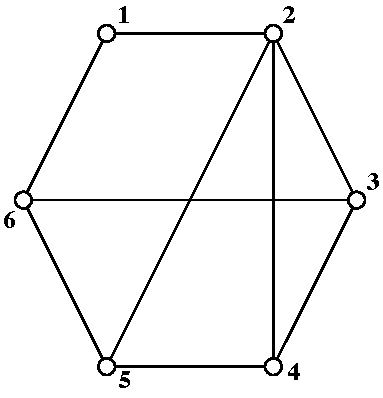
\includegraphics[width=3.5cm]{graphe_simple}
%}
%  \subfloat{
%    \centering
%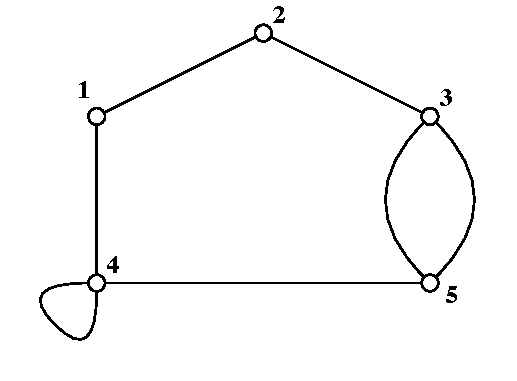
\includegraphics[width=5cm]{graphe_non_simple}
%}
%  \subfloat{
%    \centering
%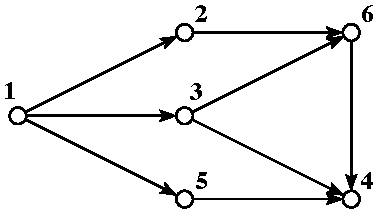
\includegraphics[width=4cm]{graphe_oriente}
%}
%\caption{Exemples de graphes : simple, avec boucle et arête multiple, orienté}\label{fig:graphes}
%\end{table}


\begin{theorem}\label{th:degre}
La somme des degr\'es d'un graphe est \'egale \`a deux fois son nombre 
d'ar\^etes. 
\end{theorem}
\bpr
Il suffit de constater que chaque arête ajoute 2 à la somme des degrés d'un graphe. 
\epr

\begin{theorem}
Le nombre de sommets de degr\'es impairs dans un graphe est pair.
\end{theorem}
\bpr
Puisque la somme des degrés est toujours paire (cf. théorème~\ref{th:degre}), le nombre d'entiers impairs dans cette somme doit être pair.
\epr


\begin{theorem}
Dans un graphe $G$ orient\'e, la somme des degr\'es entrant est \'egale
\`a la somme des degr\'es sortant et \`a son nombre d'arêtes.
\end{theorem}
\bpr
Comme pour le théorème~\ref{th:degre}, il suffit de constater que chaque arc contribue pour 1 à la somme des degrés entrant et pour 1 à celle des degrés sortants d'un graphe. 
\epr

\begin{theorem}
Le nombre maximum d'arêtes dans un graphe simple à $n$ sommets est $\frac{n \times (n  - 1)}{2}$.
\end{theorem}
\bpr
En effet, dans un graphe simple ayant un maximum d'arêtes, chaque sommet est de degré $n-1$. Par conséquent, la somme des degrés est $n \times (n-1)$ et le nombre d'arêtes $\frac{n \times (n  - 1)}{2}$.
\epr


\subsection{Graphes non étiquetés}

\subsubsection{Isomorphisme de graphes}

Deux graphes seront dits {\em isomorphes} si l'on peut passer de l'un \`a
l'autre par un simple renommage des sommets et des ar\^etes.

Plus formellement, soit deux graphes $G_1 = (V_1, E_1)$ et $G_2 = (V_2, E_2)$. $G_1$ et $G_2$ sont isomorphes si et seulement si il existe une bijection $\varphi$ de $V_1$ dans $V_2$ telle que $\forall v, w \in V_1, vw \in E_1 \Leftrightarrow  \varphi(v)\varphi(w) \in E_2$. 

Remarque :  cette notion s'applique aussi bien à des graphes orientés que non orientés.
 
Il arrive 
fr\'equemment que l'on ne fasse pas la distinction entre un graphe et
sa classe d'\'equivalence. Nous parlerons alors de {\em graphes non \'etiquet\'es}.
Inversement, l'ensemble des noms donn\'es aux sommets d'un graphe est appel\'e
un {\em \'etiquetage}.

\begin{figure}[H]
  \centering
  \subfloat{
    \centering
\begin{tikzpicture}[transform shape]

  \Vertex[x=1,y=4]{a} 
  \Vertex[x=3,y=4]{b}
  \Vertex[x=4,y=2]{c}
  \Vertex[x=3,y=0]{d} 
  \Vertex[x=1,y=0]{e}
  \Vertex[x=0,y=2]{f}

\Edge(a)(b)
\Edge(a)(f)
\Edge(b)(c)
\Edge(b)(d)
\Edge(b)(e)
\Edge(c)(d)
\Edge(c)(f)
\Edge(d)(e)
\Edge(e)(f)
\end{tikzpicture}
}
  \subfloat{
    \centering
\begin{tikzpicture}[transform shape]

  \Vertex[x=1,y=4]{a} 
  \Vertex[x=3,y=4]{b}
  \Vertex[x=4,y=2]{c}
  \Vertex[x=3,y=0]{d} 
  \Vertex[x=1,y=0]{e}
  \Vertex[x=0,y=2]{f}

\Edge(a)(b)
\Edge(a)(c)
\Edge(a)(d)
\Edge(a)(e)
\Edge(b)(d)
\Edge(b)(f)
\Edge(c)(d)
\Edge(c)(f)
\Edge(e)(f)
\end{tikzpicture}
}
\caption{Graphes isomorphes}\label{fig:isomorphisme}
\end{figure}

%\begin{figure}[hbt]
%\begin{center}
%\begin{tabular}[t]{c}
%\subfigure[]{\epsfysize=5cm\epsfbox{graphe_simple.ps}}\quad
%\subfigure[]{\epsfysize=5cm\epsfbox{isomorphe.ps}}
%\end{tabular}
%\end{center}
%\caption{Graphes isomorphes}
%\label{fig:isomorphisme}
%\end{figure}

\subsubsection{Exemple}
Les deux graphes de la figure~\ref{fig:isomorphisme} sont isomorphes,
l'isomorphisme \'etant le suivant~: $\{(a,e), (b,a), (c,c), (d,d), (e,b), (f,f)\}$.



\subsection{Chaînes}

\subsubsection{Notions non orientées}

Une {\em chaîne} est une séquence alternée de sommets et d'arêtes $P_k = v_1, e_1, v_2, \ldots, v_k, e_k, v_{k+1}$, où chaque arête $e_i$ a pour extrémités $v_i$ et $v_{i+1}$. On dira que $P_k$ est une chaîne de {\em longueur} $k$ reliant $v_1$ à $v_{k+1}$. $v_1$ et $v_{k+1}$ seront appelés les {\em extrémités} de la chaîne $P_k$.

Si $k > 0$ et $v_1 = v_{k+1}$, on dit que $P_k$ est fermée.
 
Une {\em chaîne simple} est une chaîne ne passant pas deux fois par la même arête.

Une {\em chaîne élémentaire} est une chaîne ne passant pas deux fois par le même sommet. Une chaîne élémentaire est donc forcément simple.

Un {\em cycle} est une chaîne simple fermée, c'est à dire une chaîne simple $C_k = v_1, e_1, v_2, \ldots, v_k, e_k, v_{k+1}$, telle que $v_{k+1} = v_1$.

Un {\em cycle élémentaire} est une chaîne simple fermée dont tous les sommets sont distincts à l'exception de ses extrémités.

Si le graphe $G$ est simple, il n'est pas nécessaire de préciser l'arête entre deux sommets consécutifs dans une chaîne ou un cycle. Dans ce cas, la chaîne sera donc exprimée comme une simple suite de sommets $v_1, \ldots, v_{k+1}$ ayant comme propriété que deux sommets consécutifs sont toujours voisins.

\subsubsection{Notions orientées}

Un {\em chemin} est une séquence alternée de sommets et d'arcs \\$P_k = v_1, e_1, v_2, \ldots, v_k, e_k, v_{k+1}$, où chaque arc $e_i$ a pour extrémité initiale $v_i$ et extrémité terminale $v_{i+1}$. De même que pour les chaînes, on dira que $P_k$ est un chemin de {\em longueur} $k$ reliant $v_1$ à $v_{k+1}$. 

De même qu'à une chaîne correspond la notion orientée de chemin, à chaîne simple, chaîne élémentaire, cycle, cycle élémentaire, correspondent les notions orientées de {\em chemin simple}, {\em chemin élémentaire}, {\em circuit}, {\em circuit élémentaire}.

\subsubsection{Exemples}

%\begin{figure}[H]
%\begin{center}
%\begin{tikzpicture}
%  \tikzstyle{sommet}=[circle, draw=black, fill=white, thick]
%  \node[sommet] (a) at (-1,2) {a};
%  \node[sommet] (b) at (1,3.5) {b}
%    edge [thick] (a){$e_1$};
%   \node[sommet] (c) at (3,2) {c}
%    edge [thick](b){$e_2$};
%    \node[sommet] (d) at (2,0) {d}
%    edge [thick, bend right] (c){$e_3$}
%    edge [thick, bend left] (c){$e_4$};
%    \node[sommet] (e) at (0,0) {e}
%    edge  [thick] (a){$e_5$}
%    edge  [thick] (d){$e_6$}
%    edge [thick, out=180, in=240, min distance=1cm] (e){$e_7$};
%\end{tikzpicture}
%\caption{Graphe}\label{fig:Gchaines}
%\end{center}
%\end{figure}

Dans le graphe non orienté de la figure~\ref{fig:cycle}, 

\subsection{Connexité}

\subsubsection{Définitions}

Un graphe est dit {\em connexe} si et seulement si pour toute paire de sommets $u$, $v$, il existe une chaîne reliant $u$ et $v$.

Un graphe orienté est dit  {\em fortement connexe} si et seulement si pour toute paire de sommets $u$, $v$, il existe un chemin reliant $u$ à $v$.

La {\em composante connexe} d'un sommet $v$ est l'ensemble des sommets $u$ tels qu'il existe une chaîne entre $u$ et $v$. Un graphe connexe est donc un graphe ayant une seule composante connexe.

La {\em composante fortement connexe} d'un sommet $v$ d'un graphe orienté $G$ est l'ensemble des sommets $u$ de $V(G)$ tels qu'il existe un chemin de $u$ à $v$ et un chemin de $v$ à $u$. Un graphe fortement-connexe est donc un graphe ayant une seule composante fortement connexe.


\subsubsection{Arbre}

Un {\em arbre} est un graphe connexe sans cycle. Un sommet de degré 1 dans un arbre est appelé une {\em feuille}.

Une {\em forêt} est un graphe sans cycle. Autrement dit, une forêt est un graphe dont toutes les composantes connexes sont des arbres.

On peut remarquer qu'une forêt est forcément simple, une boucle ou une arête multiple étant considérées comme des cycles.

Une {\em arborescence} est un arbre dont un sommet $r$, appelé {\em racine} est distingué. Une arborescence est naturellement orientée de sa racine vers les feuilles.


\section{Sous-graphe}

\begin{definition}
Un graphe {\em partiel} de $G = (V,E)$ est un graphe $G[F] = (V,F)$ o\`u
$F$ est un sous-ensemble de $E$.
\end{definition}

\begin{definition}
Un {\em sous-graphe induit} de $G = (V,E)$ est un graphe $G(X) = (X,F)$ o\`u
$X \subseteq V$ et $F$ est l'ensemble des ar\^etes ou arcs de E ayant leurs deux extr\'emit\'es
dans $X$.
\end{definition}

\begin{figure}[htbp]
  \centering
  \subfloat[Graphe $G$\label{fig:G}] {
    \centering
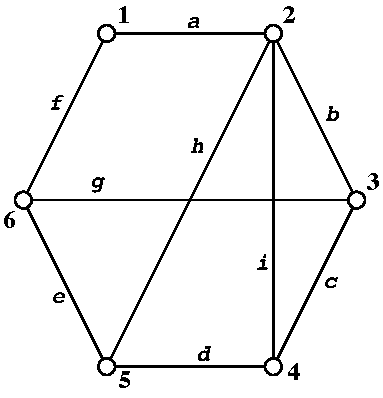
\includegraphics[height=5cm]{graphe_G}
}
\subfloat[Graphe partiel \label{fig:Gpartiel}] { %$G\[a,b,c,d\]$
    \centering
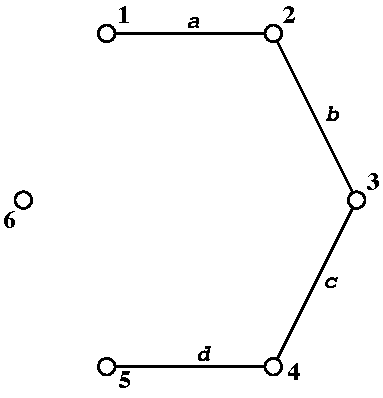
\includegraphics[width=5cm]{graphe_partiel}
}
  \subfloat[Sous-graphe induit \label{fig:Ginduit}] {
    \centering
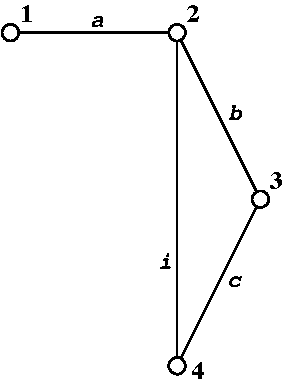
\includegraphics[height =5cm]{sous_graphe_induit}
}
\caption{Graphe $G$, graphe partiel $G[a,b,c,d]$ et sous-graphe induit $G(1,2,3,4)$}\label{fig:sous-graphes}
\end{figure}

\begin{figure}[htbp]
  \centering
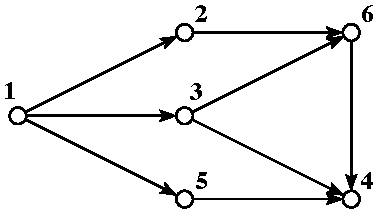
\includegraphics[width=5cm]{graphe_oriente}
\caption{Graphe orienté sans circuit}\label{fig:graphes}
\end{figure}


\paragraph{Exemples}
1,a,2,b,3,c,4 est une cha\^{\i}ne de longueur 3 du graphe de la 
figure~\ref{fig:G}.
2,b,3,c,4,d,5,h,2 est un cycle de longueur 4 de ce m\^eme graphe. Par contre,
le sous-graphe induit par $\{2,3,4,5\}$ n'est pas un cycle car il contient une
ar\^ete de trop : l'ar\^ete i. Le sous-graphe induit par $\{1, 3, 4\}$ n'est pas
connexe.\\
Le graphe de la figure~\ref{fig:graphes} ne poss\`ede aucun circuit. Le
sous-graphe induit par les sommets 1,2,6 et 4 forme un chemin de ce graphe.



\section{Zoologie}

\begin{itemize}
\item Le {\bf graphe complet} \`a $n$ sommets, not\'e ${\mathbf K_n}$, est 
le graphe simple
o\`u toute paire de sommets est reli\'ee par une ar\^ete.
\item Le {\bf cycle} ${\mathbf C_n}$ est le graphe simple connexe 
d'ordre $n$ o\`u tous les sommets sont de degr\'e 2.
\item La {\bf cha\^{\i}ne} ${\mathbf P_n}$ est l'arbre \`a $n$ sommets 
o\`u tous les sommets sont de degr\'e au plus 2.
\end{itemize}

%\begin{figure}[hbt]
%\begin{center}
%\begin{tabular}[t]{c}
%\subfigure[Arbre]{\epsfysize=3cm\epsfbox{arbre.ps}}\quad
%\subfigure[$K_5$]{\epsfysize=4cm\epsfxsize=4cm\epsfbox{K5.ps}}
%\end{tabular}
%\end{center}
%\caption{}
%\end{figure}

\begin{theorem}
La taille du graphe complet $K_n$ est $\frac{n(n-1)}{2}$.
\end{theorem}

\begin{theorem}
Soit $G$ un graphe simple d'ordre $n$ et de taille $m$. Les propri\'et\'es
suivantes sont \'equivalentes~:
\begin{enumerate}
\item $G$ est un arbre.
\item $G$ est connexe et $m = n-1$.
\item $G$ est sans cycle et $m = n-1$.
\item $G$ est connexe et toute suppression d'ar\^ete le d\'econnecte.
\item $G$ est sans cycle et tout ajout d'ar\^ete cr\'ee un cycle.
\item Entre tout couple de sommets, il existe une cha\^{\i}ne unique.
\end{enumerate}
\end{theorem}


%%%%%%%%%%%%%%%%%%%%%%%%%%%%%%%%%%

\chapter{Algorithmes}

\section{Parcours de graphes}

\subsection{Parcours en largeur}

\begin{algorithm}
\caption{Parcours en largeur PL($G,s$)}
\begin{algorithmic}[1]
\STATE $couleur(s) \leftarrow GRIS$
\STATE $d(s) \leftarrow 0$
\STATE $pere(s) \leftarrow NIL$
\STATE $F \leftarrow \{s\}$
\FORALL {$v \in V(G) \backslash {s}$} 
\STATE $couleur(v) \leftarrow BLANC$
\STATE $d(v) \leftarrow \infty$
\STATE $pere(v) \leftarrow NIL$
\ENDFOR
\WHILE {$F$ non vide}
\STATE $v   \leftarrow tete(F)$
\FORALL {$w \in Adj (v)$}
 \IF {$couleur(w) = BLANC$}
\STATE $couleur(w) \leftarrow GRIS$
\STATE $d(w) \leftarrow d(v) + 1$
\STATE $pere(w) \leftarrow v$
\STATE $Enfiler(F,w)$
\ENDIF
\ENDFOR
\STATE $Defiler(F)$
\STATE $couleur(v) \leftarrow NOIR$
\ENDWHILE
\end{algorithmic}
\end{algorithm}


\subsubsection{Complexité}


\subsection{Parcours en profondeur}

\begin{algorithm}
\caption{Parcours en profondeur PP($G$)}
\begin{algorithmic}[1]
\FORALL {$v \in V(G)$} 
\STATE $couleur(v) \leftarrow BLANC$
\STATE $pere(v) \leftarrow NIL$
\ENDFOR
\STATE $temps \leftarrow 0$
\FORALL {$v \in V(G)$} 
\IF {$couleur(v) = BLANC$}
\STATE $VisiterPP(v)$
\ENDIF
\ENDFOR
\end{algorithmic}
\end{algorithm}

\begin{algorithm}
\caption{VisiterPP($v$)}
\begin{algorithmic}[1]
\STATE $couleur(v) \leftarrow GRIS$
\STATE $d(v) \leftarrow temps \leftarrow temps + 1$
\FORALL {$w \in Adj (v)$} 
\IF {$couleur(w) = BLANC$}
\STATE $pere(w) \leftarrow v$
\STATE $VisiterPP(w)$
\ENDIF
\ENDFOR
\STATE $couleur(v) \leftarrow NOIR$
\STATE $f(v) \leftarrow temps \leftarrow temps + 1$
\end{algorithmic}
\end{algorithm}

\subsection{Applications du parcours en profondeur}

\subsubsection{Tri topologique}

Au cours d'un parcours en profondeur, à chaque fois que l'on noircit un sommet, il est inséré en tête de liste.

~\\
A $PP(G)$, rajouter une ligne {\tt 5 bis} :
\begin{algorithmic}[]
\STATE $liste \leftarrow \{\}$ 
\end{algorithmic}

~\\
A $VisiterPP(v)$, rajouter \\
trois lignes {\tt 3.1, 3.2, 3.3}
\begin{algorithmic}[]
\IF{$couleur(w) = GRIS$}
\STATE  \algorithmicreturn "Existence d'un circuit"
\ENDIF
\end{algorithmic}
une ligne {\tt 11} :
\begin{algorithmic}[]
\STATE $INSERER\_TETE(liste, v)$ 
\end{algorithmic}

\subsubsection{Composantes fortement connexes}

\begin{algorithm}
\caption{CFC($G$)}
\begin{algorithmic}[1]
\STATE Exécuter PP($G$) et trier les sommets selon un ordre décroissant de f
\STATE Calculer $G^{-1}$
\STATE Exécuter PP($G^{-1}$)
\STATE Retourner les arborescences obtenues comme composantes fortement connexes de $G$
\end{algorithmic}
\end{algorithm}

\section{Arbre de poids minimum}

\subsection{Algorithme de Kruskal}

\begin{algorithm}
\caption{Kruskal($G, w$)}
\begin{algorithmic}[1]
\FORALL {$v$ de $V(G)$} 
\STATE $composante(v) \leftarrow \{v\}$
\ENDFOR
\STATE Trier $E(G)$ dans un ordre croissant $(e_1, \ldots, e_m)$ en fonction de $w(e)$
\STATE $i \leftarrow 1$
\STATE $E(T) \leftarrow \{\}$
\WHILE {$|E(T)| < n-1$}
\IF {$e_i = (u,v)$ et $composante(u) \neq composante(v)$}
\STATE $E(T) \leftarrow E(T) \cup \{e_i\}$
\STATE UNIFIER($composante(u), composante(v)$)
\ENDIF
\STATE $i \leftarrow i+1$
\ENDWHILE
\RETURN $E(T)$
\end{algorithmic}
\end{algorithm}


\subsection{Algorithme de Prim}

\begin{algorithm}
\caption{Prim($G, w$)}
\begin{algorithmic}[1]
\STATE $F \leftarrow FILE\_PRIORITE(V(G), cle)$
\FORALL {$v$ de $V(G)$} 
\STATE $cle(v) \leftarrow \infty$
\ENDFOR
\STATE $cle(r) \leftarrow 0$
\STATE $pere(r) \leftarrow NIL$
\WHILE {$F \neq \emptyset$}
\STATE $u \leftarrow EXTRAIRE\_MIN(F)$
\FORALL {$v \in Adj(u)$}
\IF {$v \in F$ et $w(u,v) < cle(v)$}
\STATE $pere(v) \leftarrow u$
\STATE $cle(v)  \leftarrow w(u,v)$
\ENDIF
\ENDFOR
\ENDWHILE
\end{algorithmic}
\end{algorithm}

\section{Plus court chemin}

\subsection{Plus court chemin entre deux sommets}

\subsubsection{Dijkstra}

\noindent
$G$ : graphe orienté\\
$w: E(G) \rightarrow \mathbb{R}^+$ \\ 
$s$ : source de $G$

\begin{algorithm}
\caption{Dijkstra($G, w, s$)}
\begin{algorithmic}[1]
\FORALL {$v$ de $V(G)$} 
\STATE $d[v] \leftarrow \infty$
\STATE $pere[v] \leftarrow NIL$
\STATE $couleur[v] \leftarrow BLANC$
\ENDFOR
\STATE $d[s] \leftarrow 0$
\STATE $F \leftarrow FILE\_PRIORITE(V(G), d)$
\WHILE {$F \neq \emptyset$}
\STATE $pivot \leftarrow EXTRAIRE\_MIN(F)$
\STATE $couleur[pivot] \leftarrow GRIS$
\FORALL {$e = (pivot, v)$ arc sortant de $pivot$}
\IF {$couleur(v) = BLANC$ et $d[v] > d[pivot] + w(e)$}
\STATE $d[v]  \leftarrow d[pivot] + w(e)$
\STATE $pere[v]  \leftarrow pivot$
\ENDIF
\ENDFOR
\STATE $couleur[pivot] \leftarrow NOIR$
\ENDWHILE
\end{algorithmic}
\end{algorithm}


\subsubsection{Bellman}

\noindent
$G$ : graphe orienté sans circuit\\
$w: E(G) \rightarrow \mathbb{R}$ \\ 
$s$ : source de $G$


\begin{algorithm}
\caption{Bellman($G, w, s$)}
\begin{algorithmic}[1]
\FORALL {$v$ de $V(G)$} 
\STATE $d[v] \leftarrow \infty$
\STATE $pere[v] \leftarrow NIL$
\STATE $npred[v) \leftarrow deg^-[v]$
\ENDFOR
\STATE $d[s] \leftarrow 0$ 
\STATE INSERER\_FILE(F, s)
\WHILE {F non vide}
\STATE $u \leftarrow TETE\_FILE(F)$
\STATE DEFILER(F)
\FOR {$v \in Adj(u)$}
\IF {$d[v] > d[u] + w(u,v)$}
\STATE $d[v] \leftarrow d[u] + w[u,v]$
\STATE $pere[v] \leftarrow u]$
\ENDIF
\STATE $npred(v) \leftarrow nped[v] - 1$
\IF {$npred(v) = 0$}
\STATE INSERER\_FILE(F, v)
\ENDIF
\ENDFOR
\ENDWHILE
\end{algorithmic}
\end{algorithm}

\subsubsection{Algorithme de Ford}

\noindent
$G$ : graphe orienté\\
$w: E(G) \rightarrow \mathbb{R}$ \\ 
$s$ : source de $G$

L'algorithme renvoie vrai si le graphe $G$ est sans circuit.

\begin{algorithm}
\caption{PlusCourtChemin($G, w, s$)}
\begin{algorithmic}[1]
\FORALL {$v$ de $V(G)$} 
\STATE $d[v] \leftarrow \infty$
\STATE $pere[v] \leftarrow NIL$
\ENDFOR
\STATE $d[s] \leftarrow 0$ 
\FOR {$i$ de $1$ à $n-1$}
\FOR {tout arc $e \in E(G)$} 
\IF {$d[v] > d[u] + w(u,v)$}
\STATE $d[v] \leftarrow d[u] + w[u,v]$
\STATE $pere[v] \leftarrow u]$
\ENDIF
\ENDFOR
\ENDFOR
\FOR {tout arc $e \in E(G)$} 
\IF {$d[v] > d[u] + w(u,v)$}
\RETURN FAUX
\ENDIF
\ENDFOR
\RETURN VRAI
\end{algorithmic}
\end{algorithm}

\subsection{Plus courts chemins entre toutes paires de sommets}

\subsubsection{Algorithme de Floyd}

\noindent
$G$ est un graphe orienté, munis d'une fonction de poids sur les arcs $w$.\\
Les sommets sont numérotés de 1 à $n$. \\
 $W_{i,j}$ contiendra la plus courte distance entre le sommet $i$ et le sommet $j$, $Pred_{i,j}$ le sommet prédécesseur de $j$ sur un plus court chemin de $i$ à $j$.

\begin{algorithm}
\caption{Floyd($G, w$)}
\begin{algorithmic}[1]
\FOR {$i$ de $1$ à $n$}
\FOR {$j$ de $1$ à $n$}
\IF {$i = j$}
\STATE $W(i,j) \leftarrow  0$
\STATE $Pred(i,j) \leftarrow  i$
\ELSIF {$ij \in E(G)$}
\STATE $W(i,j) \leftarrow  w(i,j)$
\STATE $Pred(i,j) \leftarrow  i$
\ELSE  
\STATE $W(i,j) = \infty$
\STATE $Pred(i,j) \leftarrow  NIL$
\ENDIF
\ENDFOR
\ENDFOR
\FOR {$k$ de $1$ à $n$}
\FOR {$i$ de $1$ à $n$}
\FOR {$j$ de $1$ à $n$}
\IF {$W(i,k) + W(k,j) < W(i,j)$} 
\STATE $W(i,j) \leftarrow W(i,k) + W(k,j)$
\STATE $Pred(i,j) \leftarrow  Pred(k,j)$
\ENDIF
\ENDFOR
\ENDFOR
\ENDFOR
\end{algorithmic}
\end{algorithm}

\subsubsection{Algorithme de Warshall}

L'algorithme de Warshall est une adaptation de l'algorithme de Floyd au calcul de la fermeture transitive d'un graphe orienté. $W_{i,j}$ vaudra 1 s'il existe un chemin de $i$ à $j$ dans le graphe $G$, 0 sinon.

\begin{algorithm}
\caption{Warshall($G, w$)}
\begin{algorithmic}[1]
\FOR {$i$ de $1$ à $n$}
\FOR {$j$ de $1$ à $n$}
\IF {$i = j ~ || ~ ij \in E(G)$}
\STATE $W(i,j) \leftarrow 1$
\ELSE  
\STATE $W(i,j) = 0$
\ENDIF
\ENDFOR
\ENDFOR
\FOR {$k$ de $1$ à $n$}
\FOR {$i$ de $1$ à $n$}
\FOR {$j$ de $1$ à $n$}
\STATE $W(i,j) \leftarrow (W(i,k) ~\& ~ W(k,j)) ~\| ~ W(i,k)$
\ENDFOR
\ENDFOR
\ENDFOR
\end{algorithmic}
\end{algorithm}


\newpage

\section{Flots}


\subsection{Algorithme de Ford et Fulkerson}

\noindent
$G$ : graphe orienté\\
$c: E(G) \rightarrow \mathbb{R^+}$ \\ 
$s$ : source de $G$\\
$t$ : puit de $G$

\noindent
On considère un arc $(t,s)$ de capacité $c(t,s)$ infinie. La valeur du flot sur cet arc sera la "valeur du flot de $s$ à $t$".

\noindent
On note respectivement par $I(e)$ et $T(e)$ l'extrémité initiale et l'extrémité terminale d'un arc $e$.

\begin{algorithm}
\caption{FlotMax($G, c, s, t$)}
\begin{algorithmic}[1]
\FORALL {$e$ de $E(G)$} 
\STATE $f[e] \leftarrow 0$
\ENDFOR
\REPEAT
\STATE Marquage($G, c, f, s, t$)
\IF {$t \in Y$}  
\STATE $v \leftarrow t$
\STATE $C^+ \leftarrow \{(t,s)\}$
\STATE $C^- \leftarrow \emptyset$
\WHILE {$v \neq s$}
\STATE $e \leftarrow A[v]$
\IF {$v = T[e]$}
\STATE $C^+ \leftarrow C^+ \cup \{e\}$
\STATE $v \leftarrow I[e]$
\ELSE
\STATE $C^- \leftarrow C^- \cup \{e\}$
\STATE $v \leftarrow T[e]$
\ENDIF
\ENDWHILE
\ENDIF
\FORALL {$e \in C^+$} 
\STATE $f(e) \leftarrow f(e) + \delta[t]$
\ENDFOR
\FORALL {$e \in C^-$} 
\STATE $f(e) \leftarrow f(e) - \delta[t]$
\ENDFOR
\UNTIL{$t \not\in Y$}
\end{algorithmic}
\end{algorithm}

\begin{algorithm}
\caption{Marquage($G, c, f, s, t$)}
\begin{algorithmic}[1]
\STATE $Y \leftarrow \{s\}$
\STATE $\delta(s) \leftarrow +\infty$
\STATE $Max \leftarrow $ faux
\WHILE {$t \not\in Y et Max = $faux}
\IF {il existe $e = (u, v)$ avec $u \in Y, v \not\in Y, f(e) < c(e)$} 
\STATE $Y \leftarrow Y \cup \{v\}$
\STATE $A[v] \leftarrow e$
\STATE $\delta[v] \leftarrow min(\delta[u], c(e) -f(e))$
\ELSE \IF {il existe $e = (u, v)$ avec $v \in Y, u \not\in Y, f(e) > 0$} 
\STATE  $Y \leftarrow Y \cup \{u\}$
\STATE $A[u] \leftarrow e$
\STATE $\delta[u] \leftarrow min(\delta[v], f(e))$
\ELSE 
\STATE Max $\leftarrow vrai$ 
\ENDIF
\ENDIF
\ENDWHILE
\end{algorithmic}
\end{algorithm}

\nocite{CLRS09, CLRS10, Xuo92, CGH97, GM09, Even79, Saka84}

\bibliographystyle{unsrt}
\bibliography{bibliographie}



\end{document}

